\chapter{Background}\label{ch:background}
This chapter present more detailed introduction to solar \gls{PV} and \gls{PVS} in section \ref{sec:general_intro}. The following is context of \gls{HIL} and its applications and advantages in section \ref{sec:HIL}. 
\section{General Introduction}\label{sec:general_intro}
\gls{PVS} is type of power system which convert solar power into electricity by means of photovoltaic effect. \gls{PVS} have many advantages and become more and more popular nowadays compared with traditional fossil fuel based energy generation method. It has became a vital part of renewable energy or green energy, since it generate zero green house gas during operation. The module or panel price have experienced huge decline since middle of 2008\cite{Bazilian2013329}, which makes the the whole \gls{PV} industry prospered. According to the literature, \gls{PV} cell is able to become an important alternate renewable energy source till 2040\cite{RN3}. 
\begin{figure}[b]
    \centering
    \includegraphics[width = 0.6\textwidth]{figures/pv.png}
    \caption{Typical PV system block diagram}
    \label{fig:typical pv system}
\end{figure}

Power electronic is a vital part for solar power generation. Typically, a \gls{SSGPVC} consist of a solar panel which absorb and convert sunlight into electricity and one or more stages of power converters that transform the electricity from \gls{DC} into \gls{AC}, as well as other accessories for mounting and connecting different components. \Vref{fig:typical pv system} indicate a general configuration of \gls{PVS}. Due to the output characteristic of a typical solar cell and the need to inject power into the grid, there are at least two stages in a grid-connected PVS conventionally. The use of optional DC/DC convert(s) is to extract maximum power from upstream solar cells or units, of which is also known as \gls{MPPT}. Additionally, it is able to provide required voltage for next stage inverter to work with a appropriate duty cycle. The functionality of DC/AC converter is to inject sinusoidal current whose phase may or may not be synchronized with grid voltage(depends on applications) into grid. 

Currently, there are various configurations for grid-connected \gls{PVS} including centralized structure, the string structure, the multi-string structure and ac-module structure.\cite{5540302}. Especially, multi-string and ac-module structure have been used in a broad range of applications. Although multi-string configuration have many advantages like reducing loss due to solar panel unbalanced and a centralized \gls{MPPT} over centralized configuration, it also suffers from lacking redundancy and scalability. With optional DC/DC converter, the overall system efficiency is compromised compared with a \gls{SSGPVC}. 

As a result, ac-module configuration which is based on \gls{SSGPVC} is gaining more and more attention. The ac-module configuration is consist of only one power electronics devices which can integrate \gls{MPPT} function and convert \gls{DC} into \gls{AC} at the same time. Current design of \gls{PVS} requires for simplicity, modularity and efficiency. Those requirements are exactly the advantages of the single stage system. However, there are some issues related to the grid-connected system. The sinusoid power injected into the grid caused by the fluctuation in the dc link is one of the issue.\cite{5200525} It can force the \gls{MPPT} function to be voided so that the system can not operate at the maximum power point. Due to complexity of such converter and power rating limitations, \gls{SSGPVC} is often used in residential PV system. 

Although the \gls{SSGPVC} has some limitations, it is worth to improve the system performance and make it a better solution. Its 'apply and plug' characteristic can be consider to be a general solution to various grid-connected \gls{PV} applications. 

\section{Hardware-in-the-loop Simulation}\label{sec:HIL}
Nowadays, the complexity of various digital algorithms for power electronic applications, circuit topology is rising incredibly, which makes the simulation and development of power electronics related product increasingly time-consuming.\cite{7497546} In order to fulfill the need for fast prototyping, verified the controller functionalities without implementation of hardware, and avoid hazardous situation while testing the controller on a real hardware, the \gls{HIL} simulation or more specific \gls{PIL} simulation is deployed and used intensively for such applications. 

High-performance embedded system enabled a power electronic revolution. The increasing demand for digital controlled power electronics system requires the development to verify the controller functionalities before the controllers are tested on a real hardware platform. \gls{PIL} allow developers test and verify processors' performance on a simulator which host the virtual hardware, so it become a crucial part of developing a digital controlled power electronics system.  
\begin{figure}[b]
    \centering
    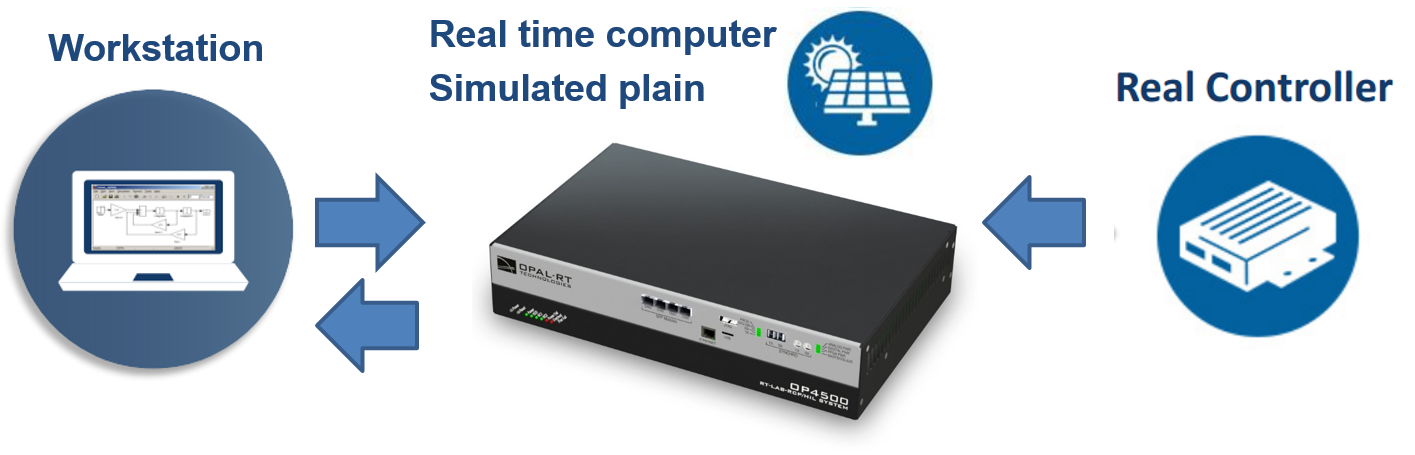
\includegraphics[width = 0.8\textwidth]{figures/pil.png}
    \caption{The basic PIL system}
    \label{fig:pil sys}
\end{figure}

Compared with traditional \gls{SIL} simulation, \gls{HIL} and \gls{PIL} simulation is another level of simulation which runs way faster than the \gls{SIL} simulation. In conventional \gls{SIL} simulation for power electronics application, the time it takes to run the simulation is often longer than the simulation time span of interest, which means, for example,  people need to speed more than one second in order to generate one second of results. On the contrary, the \gls{HIL} and \gls{PIL} simulation run in real-time without sacrificing simulation time step resolution. If one second is spent on the simulation process, results for one second can be generated with corresponding resolution that preserves all the transient state of prototype under simulation. 

Comparing \gls{HIL} simulation with \gls{PIL} simulation, the \gls{PIL} simulation offers a more close-to-real results since in many applications the functionalities needed is hard to abstract and model using software. In \gls{PIL} simulation, the controller functionalities are executed inside by a real controller, so the developers do not need to worry about how to implement a precise controller model inside software environment.

Fig.\ref{fig:pil sys} illustrate a basic setup for \gls{PIL} simulation. The power converter operate inside the \gls{RT} computer. There are  multiple ways that the real controller can communicate with the \gls{RT} simulator. The simulator is capable of generating necessary voltage or current signal through \gls{DAC} so that the external controller can sense the signal and generate proper trig signal feeding back to the \gls{RT} computer. The \gls{RT} computer also have \gls{GPIO} to read all the controller generated signal and carry them into runtime simulation. Another way mentioned in this papar\cite{7497546} is to use direct file exchange and there is a solution support this method with any type of controller architecture. 

For the sake of running \gls{PIL} simulation, a power converter testbed needed to be implement inside the software environment. The \gls{RT} computer has equipped with a powerful \gls{CPU} as well as \gls{FPGA} acceleration card. For the sake of fully utilize the computation power of the simulator, the model should be construct complying to some rules and regulations. But converting an existing converter model into \gls{RT} simulation compatible model requires a bit of work and experience which is described in detailed in chapter \ref{ch:implementation}.

\section{Previous work}
\gls{PIL} simulation has been used for \gls{PV} application. In paper,\cite{RN11} a two stages \gls{PVS} was implemented using RT-LAB which is a software for controlling the \gls{RT} simulator. In this paper, the simulation setup compose of a solar panel model, a grid-connected inverter and a DC/DC converter in the software environment. Also, there is a physical controller controlling DC/DC converter so that the author could perform \gls{PIL} simulation. This paper proves that it is feasible to use \gls{PIL} for \gls{PVS} simulation and gave a detailed example of how to implement \gls{RT} simulation model using the corresponding software. The major improvement to the results of the paper would improving the \gls{PWM} frequency of the controller since the state-of-art digital controlled converter's \gls{PWM} can be as high as a few mega hertz while in the paper the \gls{PWM} frequency is only 10 kHz. Also, making use of the \gls{FPGA} acceleration card in the \gls{RT} simulator would be beneficial to provide finer time resolutions and enable higher \gls{PWM} processing capabilities.

Many researchers have already completed lots of research work regarding \gls{SSGPVC} as well as PV panels as a whole system. In particular, Paper \cite{RN3} presents approaches on modeling of single stage \gls{PVS} for \gls{RT} simulation. This paper focus on discrete time modeling of the whole system, while at the same time it proposed a new MPPT method which is based on \gls{IC} and had the new algorithm tested using \gls{RT} simulation. In this paper, the author had the \gls{RT} simulator investigated and concluded that the \gls{RT} simulators have sufficient computation power to perform simulation for PV applications. 